% proj3.tex
% Filip Kocica [xkocic01@fit.vutbr.cz]
% ITY - Tabulky a obrazky
% 21/3/2017

\documentclass[11pt, titlepage, a4paper]{article}
\usepackage[left=1.5cm,text={17cm, 24cm},top=3cm,left=2cm]{geometry}
\usepackage[czech]{babel}
\usepackage[utf8]{inputenc}
\usepackage[T1]{fontenc}
\usepackage{times}
\usepackage[ruled,czech,linesnumbered,longend,noline]{algorithm2e}
\usepackage{algorithmic}
\usepackage{graphics}
\usepackage{picture}
\usepackage{pdflscape}

\begin{document}

		\begin{titlepage}
    \begin{center}
		\textsc{\Huge{Vysoké učení technické v~Brně\\}
		\huge{Fakulta informačních technologií\\}}
		\vspace{\stretch{0.382}}
		\LARGE{Typografie a~publikování -- 3. projekt\\}
		\Huge{Tabulky a~obrázky\\}
		\vspace{\stretch{0.618}}
		\end{center}
		\Large{21.března 2017 \hfill Filip Kočica}
		\end{titlepage}

%   section - uvodni strana
		\section{Úvodní strana}
			Název práce umístěte do zlatého řezu a~nezapomeňte uvést dnešní datum a~vaše jméno
			a~příjmení.

		  \section{Tabulky}
			  Pro sázení tabulek můžeme použít buď prostředí  \texttt{ tabbing }  nebo prostředí
			   \texttt{ tabular.}

		  \subsection{Prostředí  \texttt{ tabbing }}
			  Při použití  \texttt{ tabbing }  vypadá tabulka následovně:

	    \begin{tabbing}
      ovoce XYZ ~~~~~~~~~\= cena ~~~~
      \= 34 \kill
      \bfseries \textbf{Ovoce} \>
      \bfseries \textbf{Cena} \>
      \bfseries \textbf{Množství} \\[1mm]
      Jablka \> 25,90 \> 3 kg\\
      Hrušky \> 27,40 \> 2,5 kg\\
      Vodní melouny \> 35,-- \> 1 kus
      \end{tabbing}

		  \noindent
		  Toto prostředí se dá také použít pro sázení algoritmů, ovšem vhodnější je použít
		  prostředí  \texttt{ algorithm }  nebo  \texttt{ algorithm2e }  (viz sekce
		  \ref{sec:alg}).

		  \subsection{Prostředí  \texttt{ tabular}}
			  Další možností, jak vytvořit tabulku, je použít prostředí  \texttt{ tabular. } Tabulky
			  pak budou vypadat asi takto\footnotemark[1]:

		  \bigskip
		  \begin{table}[h]
		  \begin{center}
		  \catcode`\-=12
		  \begin{tabular}{|c|r|r|} \hline
        & \multicolumn{2}{|c|}{\textbf{Cena}}\\\cline{2-3}
        \textbf{Měna} & \textbf{nákup} & \textbf{prodej}\\ \hline
      	EUR & 27,02 & 27,20\\
     		GBP & 31,08 & 31,80\\
   		  USD & 25,15 & 25,51\\ \hline
		  \end{tabular}
		  \caption{Tabulka kurzů k~dnešnímu dni}
		  \label{tab:mena}
		  \end{center}
		  \end{table}

      \bigskip
      \begin{table}[h]
      \begin{center}
      \catcode`\-=12
      \begin{tabular}{|c|c|} \hline
        $A$ & $\neg A$\\ \hline
        \textbf{P} & N\\ \hline
        \textbf{O} & O\\ \hline
        \textbf{X} & X\\ \hline
        \textbf{N} & P\\ \hline
      \end{tabular}
            \begin{tabular}{|c|c|c|c|c|c|} \hline
        \multicolumn{2}{|c|}{$A \wedge B$} & \multicolumn{4}{|c|}{$B$}\\ \cline{3-6}
        \multicolumn{2}{|c|}{} & \textbf{P} & \textbf{O} & \textbf{X} & \textbf{N}\\ \hline
        & \textbf{P} & P & O & X & N\\ \cline{2-6}
        A & \textbf{O} & O & O & N & N\\ \cline{2-6}
        & \textbf{X} & X & N & X & N\\ \cline{2-6}
        & \textbf{N} & N & N & N & N\\ \hline
      \end{tabular}
      \begin{tabular}{|c|c|c|c|c|c|} \hline
        \multicolumn{2}{|c|}{$A \vee B$} & \multicolumn{4}{|c|}{$B$}\\ \cline{3-6}
        \multicolumn{2}{|c|}{} & \textbf{P} & \textbf{O} & \textbf{X} & \textbf{N}\\ \hline
        & \textbf{P} & P & P & P & P\\ \cline{2-6}
        A & \textbf{O} & P & O & P & O\\ \cline{2-6}
        & \textbf{X} & P & P & X & X\\ \cline{2-6}
        & \textbf{N} & P & O & X & N\\ \hline
      \end{tabular}
      \begin{tabular}{|c|c|c|c|c|c|} \hline
        \multicolumn{2}{|c|}{$A \rightarrow B$} & \multicolumn{4}{|c|}{$B$}\\ \cline{3-6}
        \multicolumn{2}{|c|}{} & \textbf{P} & \textbf{O} & \textbf{X} & \textbf{N}\\ \hline
        & \textbf{P} & P & O & X & N\\ \cline{2-6}
        A & \textbf{O} & P & O & P & O\\ \cline{2-6}
        & \textbf{X} & P & P & X & X\\ \cline{2-6}
        & \textbf{N} & P & P & P & P\\ \hline
      \end{tabular}
      \caption{Protože Kleeneho trojhodnotová logika už je \uv{zastaralá}, uvádíme si zde příklad
				čtyřhodnotové logiky}
      \label{tab:kleen}
      \end{center}
      \end{table}

		  \footnotetext[1]{Kdyby byl problém s~\texttt{ cline, } zkuste se podívat třeba sem:
			  http://www.abclinuxu.cz/tex/poradna/show/325037.}

		  \newpage

%   section - algoritmy
		\section{Algoritmy}
      \label{sec:alg}
			Pokud budeme chtít vysázet algoritmus, můžeme použít prostředí \texttt{ algorithm}
			\footnotemark[2]  nebo \texttt{ algorithm2e}\footnotemark[3].
			Příklad použití prostředí \texttt{ algorithm2e } viz Algoritmus \ref{alg}.

		  \algsetup{indent=2em}
		  \begin{algorithm}[h]
		  \caption{\textsc{Fast}SLAM}
		  \label{alg}
		  \SetKwInput{Input}{Input}
		  \Input{$(X_{t-1},u_t,z_t)$}
		  \SetKwInOut{Output}{Output}
		  \Output{$X_t$}
		  \SetNlSty{}{}{:  } % dvojtecka za cisly radku
		  \SetInd{1em}{1em}
		  \SetNlSkip{-1.33em}

		  \BlankLine
		  \Indp \Indp
      $\overline{X_t} = X_t = 0$\\
      \For{$k=1$ \textnormal{to} $M$}
      {
      		$x_t^{[k]} =$ \emph{sample\_motion\_model}$(u_t,x_{t-1}^{[k]})$\\
      		$w_t^{[k]} =$ \emph{measurement\_model}$(z_t,x_t^{[k]},m_{t-1})$\\
      		$m_t^{[k]} = updated\_occupancy\_grid(z_t,x_t^{[k]},m_{t-1}^{[k]})$\\
      		$\overline{X_t} = \overline{X_t} + \langle x_x^{[m]},w_t^{[m]}\rangle$
      }
      \For{$k=1$ \textnormal{to} $M$}
      {
      		draw $i$ with probability $\approx w_t^{[i]}$\\
      		add $\langle x_x^{[k]},m_t^{[k]}\rangle$ to $X_t$\\
      }
      \Return{$X_t$}
		  \end{algorithm}


%   section - obrazky
		\section{Obrázky}
			Do našich článků můžeme samozřejmě vkládat obrázky. Pokud je obrázkem fotografie,
			můžeme klidně použít bitmapový soubor. Pokud by to ale mělo být nějaké schéma nebo
			něco podobného, je dobrým zvykem takovýto obrázek vytvořit vektorově.

			\begin{figure}[h]
			\begin{center}
				\scalebox{0.4}{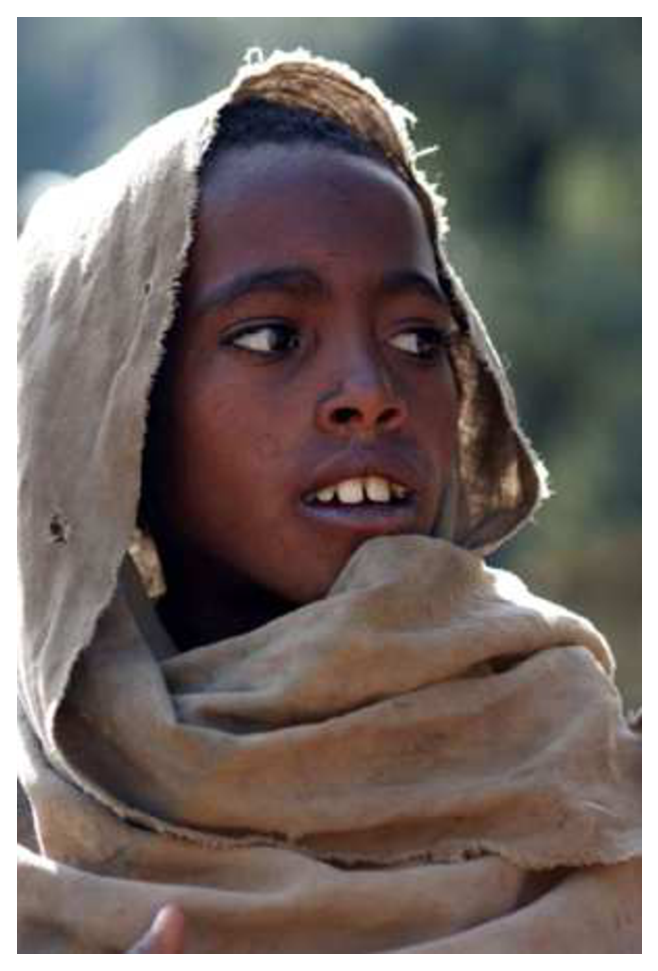
\includegraphics{etiopan.eps}
        \reflectbox{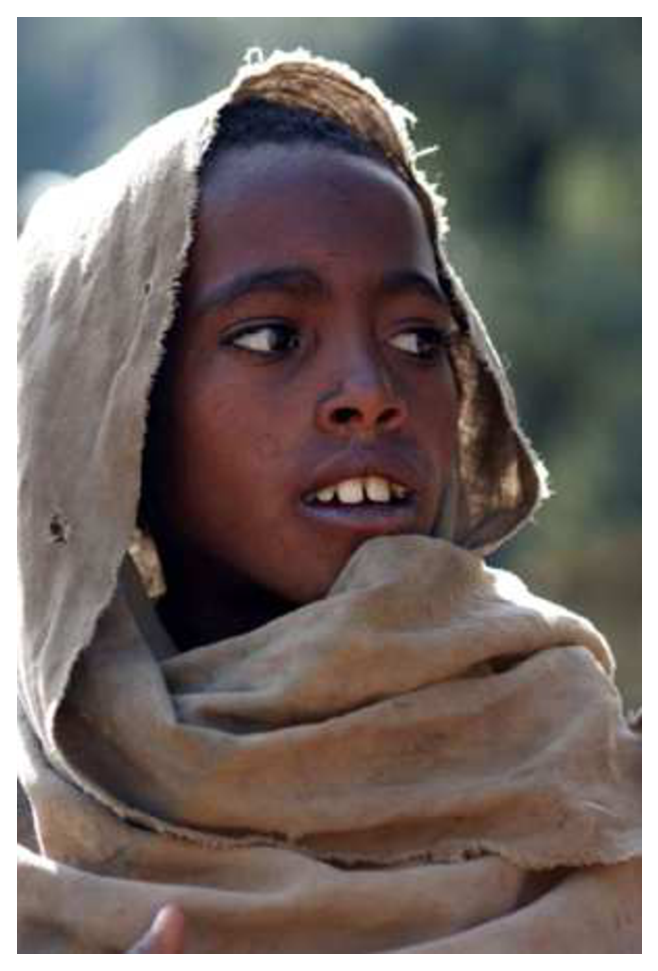
\includegraphics{etiopan.eps}}}
				\caption{Malý Etiopánek a jeho bratříček}
				\label{o:etiopan}
			\end{center}
			\end{figure}

			\footnotetext[2]{Pro nápovědu, jak zacházet s~prostředím \texttt{ algorithm, }
			můžeme zkusit tuhle stránku:\\http://ftp.cstug.cz/pub/tex/CTAN/macros/latex/contrib/
      algorithms/algorithms.pdf.}
			\footnotetext[3]{Pro \texttt{ algorithm2e } zase tuhle: http://ftp.cstug.cz/pub/tex/CTAN/
      macros/latex/contrib/algorithm2e/doc/algorithm2e.pdf.}

			\newpage
			Rozdíl mezi vektorovým \dots
			\begin{figure}[ht]
			\begin{center}
				\scalebox{0.4}{
\includegraphics{oniisan.eps}}
				\caption{Vektorový obrázek}
				\label{o:vektor}
			\end{center}
			\end{figure}

			\dots a bitmapovým obrázkem
			\begin{figure}[ht]
			\begin{center}
				\scalebox{0.6}{
\includegraphics{oniisan2.eps}}
				\caption{Bitmapový obrázek}
				\label{o:bitmap}
			\end{center}
			\end{figure}

			\noindent se projeví například při zvětšení.

			Odkazy (nejen ty) na obrázky \ref{o:etiopan}, \ref{o:vektor} a~\ref{o:bitmap}, na
			tabulky \ref{tab:mena} a~\ref{tab:kleen} a~také na algoritmus \ref{alg} jsou
			udělány pomocí křížových odkazů. Pak je ovšem potřeba zdrojový soubor přeložit dvakrát.

			Vektorové obrázky lze vytvořit i~přímo v~\LaTeX u, například pomocí
			prostředí \texttt{ picture.}

      \newpage

  \begin{landscape}
\begin{figure}
\setlength{\unitlength}{4pt}
\begin{picture}(145,75)(0,0)

        \linethickness{2pt}
        \put(15,7){\framebox(145,75)}

\end{picture}
\caption{Vektorový obrázek.}
\end{figure}
\end{landscape}
\end{document}
